\documentclass[stat333]{subfiles}

%% ========================================================
%% document

\begin{document}

    \chap{Stochastic Processes}

    \section{Stochastic Processes}

    \begin{definition}{Stochastic Process}{}
        Any collection of random variables (or random vectors) of the form $\left\lbrace X\left( t \right) \right\rbrace^{}_{t\in\mT}$ is called a \emph{stochastic process}.
    \end{definition}

    \np Given a stochastic process $\left\lbrace X\left( t \right) \right\rbrace^{}_{t\in\mT}$ The index set $\mT$ is often interpreted in the context of time. As such, usually $\mT\subseteq\R$ and we say $X\left( t \right)$ is the \emph{state} of the process at time $t\in\mT$.

    \begin{definition}{Continuous-time, Discrete-time}{Stochastic Process}
        Let $\left\lbrace X\left( t \right) \right\rbrace^{}_{t\in\mT}$ be a stochastic process. We say $\left\lbrace X \right\rbrace^{}_{t\in\mT}$ is 
        \begin{enumerate}
            \item \emph{continuous-time} if $\mT$ is a (union of) continuum of real numbers; and
            \item \emph{discrete-time} if $\mT$ is a countable subset of real numbers.\footnote{In general, we use $\N\cup\left\lbrace 0 \right\rbrace$ as the index set of discrete-time stochastic processes. In fact, we shall use this convention throughout this note, unless otherwise specified.}
        \end{enumerate}
    \end{definition}

    \begin{definition}{Discrete-time Markov Chain (DTMC)}{}
        We say a discrete-time stochastic process $\left\lbrace X_n \right\rbrace^{}_{n\in\N\cup\left\lbrace 0 \right\rbrace}$ is a \emph{discrete-time Markov chain} (\emph{DTMC}) if
        \begin{enumerate}
            \item each $X_n$ is discrete; and
            \item for every $n\in\N\cup\left\lbrace 0 \right\rbrace$ and $x_0,\ldots,x_{n+1}$ in the codomain of $X_0,\ldots,X_{n+1}$, respectively,
                \begin{equation*}
                    \PP\left( X_{n+1}=x_{n+1}|X_{n}=x_{n},\ldots,X_0=x_0 \right) = \PP\left( X_{n+1}=x_{n+1}|X_{n}=x_{n} \right).\eqno\text{\textit{Markov property}}
                \end{equation*}
        \end{enumerate}
    \end{definition}

    \np In other words, the Markov property states that the conditional distribution of a \textit{future} state $X_{n+1}$ given the \textit{past} states $X_0,\ldots,X_{n-1}$ and the \textit{present} state $X_n$ is independent of the past states. It is also worth noting that the Markov property ensures that, given any $k_1,\ldots,k_l\in\left\lbrace 1,\ldots,n-1 \right\rbrace$ with $k_1<\cdots<k_l$,
    \begin{equation*}
        \PP\left( X_{n+1}=x_{n+1}|X_{k_l}=x_{k_l},\ldots,X_{k_1}=x_{k_1} \right) = \PP\left( X_{n+1}=x_{n+1}|X_{k_l}=x_{k_l} \right).
    \end{equation*}

    \begin{definition}{Transition Probability Matrix}{}
        For any pair of states $i,j\in\N\cup\left\lbrace 0 \right\rbrace$, the \emph{transition probability} from state $i$ at time $n$ to state $j$ at time $n+1$ is given by
        \begin{equation*}
            \PP\left( X_{n+1}=j|X_n=i \right)
        \end{equation*}
        for all $n\in\N\cup\left\lbrace 0 \right\rbrace$. The \emph{transition probability matrix} from time $n$ to time $n+1$ is defined as 
        \begin{equation*}
            \begin{bmatrix}
                P_{n,0,0} & P_{n,0,1} & \cdots \\
                P_{n,1,0} & P_{n,1,1} & \cdots \\
            	\vdots & \vdots & \ddots \\
            \end{bmatrix}
        \end{equation*}
        for all $n\in\N\cup\left\lbrace 0 \right\rbrace$, where $P_{n,i,j}=\PP\left( X_{n+1}=j|X_n=i \right)$ for all $i,j\in\N\cup\left\lbrace 0 \right\rbrace$.
    \end{definition}

    \clearpage
    \np It is clear from the construction that, given any TPM $P$,
    \begin{enumerate}
        \item every entry of $P$ is nonnegative; and
        \item for any row of $P$, the sum of the entries is $1$.
    \end{enumerate}
    Any matrix that satisfies (a), (b) is called \emph{stochastic}.

    \begin{definition}{Stationary (Homogeneous)}{DTMC}
        Let $\left\lbrace X_n \right\rbrace^{}_{n\in\N\cup\left\lbrace 0 \right\rbrace}$ be a DTMC. We say $\left\lbrace X_n \right\rbrace^{}_{n\in\N\cup\left\lbrace 0 \right\rbrace}$ is \emph{stationary} (or \emph{homogeneous}) if the transition probability is independent of the time.\footnote{We shall only consider stationary DTMCs in this note.} That is, for all times $n,m\in\N\cup\left\lbrace 0 \right\rbrace$ and indices $i,j\in\N\cup\left\lbrace 0 \right\rbrace$,
        \begin{equation*}
            \PP\left( X_{n+1}=j|X_n=i \right) = \PP\left( X_{m+1}=j|X_n=i \right).
        \end{equation*}
    \end{definition}


    \ex On a given day the weather is clear, overcast, or rainy. 
    If the weather is clear today, then it would be clear, overcast, or rainy tomorrow with respective probabilities $0.6,0.3,0.1$. 
    If the weather is overcast today, then it would be clear, overcast, or rainy tomorrow with respective probabilities $0.2,0.5,0.3$. 
    If the weather is rainy today, then it would be clear, overcast, or rainy tomorrow with respective probabilities $0.4,0.2,0,4$. 
    Construct the underlying DTMC and determine its TPM.

    \begin{subproof}[Answer]
        Note that the weather tomorrow only depends on the weather today, implying that the Markov property holds. Hence, letting
        \begin{equation*}
            X_n = 
            \begin{cases} 
                0 & \text{if the weather on $n$th day is clear}\\
                1 & \text{if the weather on $n$th day is overcast}\\
                2 & \text{if the weather on $n$th day is rainy}
            \end{cases},
        \end{equation*}
        $\left( X_{n} \right)^{}_{n\in\N\cup\left\lbrace 0 \right\rbrace}$ is a $3$-state DTMC. Moreover, the TPM is given by
        \begin{equation*}
            \begin{bmatrix}
            	0.6 & 0.3 & 0.1 \\
            	0.2 & 0.5 & 0.3 \\
            	0.4 & 0.2 & 0.4 \\
            \end{bmatrix}. \eqqedsym
        \end{equation*}
    \end{subproof}

    \begin{definition}{$n$-step Transition Probability}{}
        Suppose that we have a DTMC $\left\lbrace X_n \right\rbrace^{}_{n\in\N\cup\left\lbrace 0 \right\rbrace}$. For every states $i,j\in\N\cup\left\lbrace 0 \right\rbrace$ and $n\in\N\cup\left\lbrace 0 \right\rbrace$, we define the \emph{$n$-step transition probability}, commonly denoted as $P^{\left( n \right)}_{i,j}$, as
        \begin{equation*}
            P^{\left( n \right)}_{i,j} = \PP\left( X_{m+n}=j|X_m=i \right),
        \end{equation*}
        where $m\in\N\cup\left\lbrace 0 \right\rbrace$.\footnote{The definition is independent of $m$ since we assumed our DTMC to be stationary. In other words, we may define $P^{\left( n \right)}_{i,j}=\PP\left( X_n=j|X_0=i \right)$.} We call
        \begin{equation*}
            P^{\left( n \right)} = \left[ P^{\left( n \right)}_{i,j} \right]_{i,j\in\N\cup\left\lbrace 0 \right\rbrace}
        \end{equation*}
        the \emph{$n$-step transition probability matrix} (\emph{$n$-step TPM}).
    \end{definition}

    \clearpage
    \np Consider a DTMC $\left\lbrace X_n \right\rbrace^{}_{n\in\N\cup\left\lbrace 0 \right\rbrace}$, its TPM $P$, and $n$-step TPMs $P^{\left( 0 \right)}, \ldots$.
    \begin{enumerate}
        \item From the construction, it is evident that
            \begin{equation*}
                P^{\left( 0 \right)}_{i,j}=\delta_{ij}
            \end{equation*}
            for every states $i,j$, where $\delta$ is the Kronecker delta. It follows that $P^{\left( 0 \right)}$ is the identity matrix.
        \item $P^{\left( 1 \right)}=P$.
    \end{enumerate}
    
    \np[Chapman-Kolmogorov Equations]For any $n\in\N$, we have
    \begin{equation}
        P^{\left( n \right)}_{i,j} = \sum^{\infty}_{k=0}P^{\left( n-1 \right)}_{i,k}P_{k,j}.
    \end{equation}

    \begin{subproof}
        Observe that    
        \begin{flalign*}
            && P^{\left( n \right)}_{i,j} & = \PP\left( X_n=j|X_0=i \right) && \\ 
            && & = \sum^{\infty}_{k=0}\PP\left( X_n=j|X_{n-1}=k,x_0=i \right)\PP\left( X_{n-1}=k|X_0=i \right) && \\
            && & = \sum^{\infty}_{k=0}P^{\left( n-1 \right)}_{i,k}\PP\left( X_n=j|X_{n-1}=k,X_0=i \right) && \\
            && & = \sum^{\infty}_{k=0}P^{\left( n-1 \right)}_{i,k}\PP\left( X_n=j|X_{n-1}=k \right) && \text{by Markov property}\\
            && & = \sum^{\infty}_{k=0}P^{\left( n-1 \right)}_{i,k}P_{k,j}, 
        \end{flalign*} 
        as required.
    \end{subproof}
    
    \noindent This in particular implies that,
    \begin{equation}
        P^{\left( n \right)} = P^{\left( n-1 \right)}P
    \end{equation}
    for every $n\in\N$, and as a corollary,
    \begin{eqbox}[Chapman-Komogorov Equations for a DTMC]
        \begin{equation}
            P^{\left( n \right)}_{i,j} = \sum^{\infty}_{k=0}P^{\left( m \right)}_{i,k}P^{\left( n-m \right)}_{k,j}
        \end{equation}
    \end{eqbox} 
    for every $i,j\in\N\cup\left\lbrace 0 \right\rbrace$ and $n\in\N, m\in\left\lbrace 0,\ldots,n \right\rbrace$. In matrix form, this translates to
    \begin{eqbox}[Chapman-Komogorov Equations in Matrix Form]
        \begin{equation}
            P^{\left( n \right)} = P^{\left( m \right)}P^{\left( n-m \right)}.
        \end{equation}
    \end{eqbox} 

    \np Consider the row vector
    \begin{equation*}
        \alpha_n = \begin{bmatrix} \alpha_{n,0} & \alpha_{n,1} & \cdots  \end{bmatrix}
    \end{equation*}
    for every $n\in\N\cup\left\lbrace 0 \right\rbrace$, where
    \begin{equation*}
        \alpha_{n,k} = \PP\left( X_n=k \right)
    \end{equation*}
    for every $k\in\N$. In other words, $\alpha_n$ represents the marginal pmf of $X_n$, and as a consequence,
    \begin{equation*}
        \sum^{\infty}_{k=0}\alpha_{n,k} = 1.
    \end{equation*}
    In case $n=0$, $\alpha_0$ is referred to as the \emph{initial conditions} (or \emph{initial probability row vector}) of the DTMC. Now let us see how we can calculate $\alpha_n$. For every $n\in\N, m\in\left\lbrace 0,\ldots,n \right\rbrace$, note that
    \begin{flalign*}
        && \alpha_{n,k} & = \PP\left( X_n=k \right) && \\ 
        && & = \sum^{\infty}_{i=0}\PP\left( X_n=k|X_m=i \right)\PP\left( X_m=i \right) && \\
        && & = \sum^{\infty}_{i=0}\alpha_{m,i}\PP\left( X_{n-m}=k|X_0=i \right) && \text{since the DTMC is stationary} \\
        && & = \sum^{\infty}_{i=0}\alpha_{m,i}P_{i,k}^{\left( n-m \right)}.
    \end{flalign*} 
    In matrix form,
    \begin{equation*}
        \alpha_n = \alpha_mP^{\left( n-m \right)} = \alpha_mP^{n-m},
    \end{equation*}
    or
    \begin{eqbox}[Marginal PDF of $X_n$]
        \begin{equation}
            \alpha_n = \alpha_0P^n.
        \end{equation}
    \end{eqbox} 

    \np Having knowledge of the initial conditions and the one-step transition probabilities, one can calculate various probabilites of possible interest, such as
    \begin{flalign*}
        && \PP\left( X_n=x_n, \ldots, X_0=x_0 \right)& = \PP\left( X_0=x_0 \right)\PP\left( X_1=x_1|X_0=x_0 \right)\cdots\PP\left( X_n=x_n|X_{n-1}=x_{n-1},\ldots,X_0=x_0 \right) && \\ 
        && & = \PP\left( X_0=x_0 \right)\PP\left( X_1=x_1|X_0=x_0 \right)\cdots\PP\left( X_n=x_n|X_{n-1}=x_{n-1} \right) && \\
        && & = \alpha_{0,x_0}P_{x_0,x_1}\cdots P_{x_{n-1},x_n}. 
    \end{flalign*} 
    Similarly,
    \begin{flalign*}
        && & \PP\left( X_{n+m}=x_{n+m},\ldots,X_{n+1}=x_{n+1}|X_n=x_n \right) && \\
        && & = \frac{\PP\left( X_{n+m}=x_{n+m},\ldots,X_n=x_n \right)}{\PP\left( X_n=x_n \right)} && \\ 
        && & = \frac{\PP\left( X_n=x_n \right)\PP\left( X_{n+1}=x_{n+1}|X_n=x_n \right)\cdots\PP\left( X_{n+m}=x_{n+m}|X_{n+m-1}=x_{n+m-1},\ldots,X_n=x_n \right)}{\PP\left( X_n=x_n \right)} && \\
        && & = P_{x_n,x_{n+1}}\cdots P_{x_{n+m-1},x_{n+m}}.
    \end{flalign*} 
    The key observation is that the DTMC is \textit{completely characterized} by its one-step TPM $P$ and the initial conditions $\alpha_0$.
    
    \ex A particle moves along the states $0,1,2$ according to a DTMC whose TPM $P$ is given by
    \begin{equation*}
        P = 
        \begin{bmatrix}
        	0.7 & 0.2 & 0.1 \\
        	0 & 0.6 & 0.4 \\
        	0.5 & 0 & 0.5 \\
        \end{bmatrix}.
    \end{equation*}
    Let $X_n$ denote the position of the particle after the $n$th move (i.e. the DTMC is $\left\lbrace X_n \right\rbrace^{}_{n\in\N\cup\left\lbrace 0 \right\rbrace}$). Suppose that the particle is equally likely to start in any of the three positions.
    \begin{enumerate}
        \item Calculate $\PP\left( X_3=1|X_0=0 \right)$.

            \begin{subproof}[Answer]
                We desire to find $P_{0,1}^{\left( 3 \right)}$. To get this, we proceed to calculate $P^{\left( 3 \right)}$, the $3$-step transition TPM, which satisfies
                \begin{equation*}
                    P^{\left( 3 \right)} = P^3
                \end{equation*}
                where $P$ is the TPM. First of all,
                \begin{equation*}
                    P^2 = 
                    \begin{bmatrix}
                    	0.54 & 0.26 & 0.2 \\
                    	0.2 & 0.36 & 0.44 \\
                    	0.6 & 0.1 & 0.3 \\
                    \end{bmatrix}
                \end{equation*}
                and
                \begin{equation*}
                    P^3 = 
                    \begin{bmatrix}
                    	0.478 & 0.264 & 0.258 \\
                    	0.36 & 0.256 & 0.384 \\
                    	0.57 & 0.18 & 0.25 \\
                    \end{bmatrix}
                \end{equation*}
                by direct calculations. Thus,
                \begin{equation*}
                    P_{0,1}^{\left( 3 \right)} = P_{0,1}^3 = 0.264. \eqqedsym
                \end{equation*}
            \end{subproof}

        \item Calculate $\PP\left( X_4=2 \right)$.

            \begin{subproof}[Answer]
                We desire to find
                \begin{equation*}
                    \alpha_{4,2} = \PP\left( X_4=2 \right).
                \end{equation*}
                To do so, let us calculate $\alpha_4$, which satisfies
                \begin{equation*}
                    \alpha_4 = \alpha_0P^4.
                \end{equation*}
                By a direct calculation,
                \begin{equation*}
                    P^4 = 
                    \begin{bmatrix}
                    	\frac{1159}{2500} & \frac{127}{500} & \frac{353}{1250} \\
                    	\frac{111}{250} & \frac{141}{625} & \frac{413}{1250} \\
                    	\frac{131}{250} & \frac{111}{500} & \frac{127}{500} \\
                    \end{bmatrix},
                \end{equation*}
                so
                \begin{equation*}
                    \alpha_4 = \alpha_0P^4 = \begin{bmatrix} \frac{1}{3} & \frac{1}{3} & \frac{1}{3} \end{bmatrix}
                    \begin{bmatrix}
                    	\frac{1159}{2500} & \frac{127}{500} & \frac{353}{1250} \\
                    	\frac{111}{250} & \frac{141}{625} & \frac{413}{1250} \\
                    	\frac{131}{250} & \frac{111}{500} & \frac{127}{500} \\
                    \end{bmatrix}
                    =
                    \begin{bmatrix} \frac{1193}{2500} & \frac{877}{3750} & \frac{2167}{7500} \end{bmatrix}.
                \end{equation*}
                Thus
                \begin{equation*}
                    \alpha_{4,2} = \frac{2167}{7500}. \eqqedsym
                \end{equation*}
            \end{subproof}

        \item Calculate $\PP\left( X_6=0, X_4=2 \right)$.

            \begin{subproof}[Answer]
                We have
                \begin{equation*}
                    \PP\left( X_6=0, X_4=2 \right) = \PP\left( X_4=2 \right)\PP\left( X_6=0|X_4=2 \right) = \alpha_{4,2}P^{\left( 2 \right)}_{2,0} = 0.17336. \eqqedsym
                \end{equation*}
            \end{subproof}

        \item Calculate $\PP\left( X_9=0, X_7=2|X_5=1, X_2=0 \right)$.

            \begin{subproof}[Answer]
                We have
                \begin{flalign*}
                    && & \PP\left( X_9=0, X_7=2|X_5=1, X_2=0 \right) && \\
                    && & = \PP\left( X_7=2|X_5=1,X_4=0 \right)\PP\left( X_9=0|X_7=2,X_5=1,X_2=0 \right)  && \\
                    && & = \PP\left( X_7=2|X_5=1 \right)\PP\left( X_9=0|X_7=2 \right) = P^{\left( 2 \right)}_{1,2}P^{\left( 2 \right)}_{2,0} = 0.264.&&\fqqedsym
                \end{flalign*} 
            \end{subproof}
    \end{enumerate}

    \section{Accessibility and Communication}
    
    \begin{definition}{Accessble}{State}
        Let $i,j$ be states of a DTMC with $n$-step TPMs $P^{\left( n \right)}$.
        \begin{enumerate}
            \item We say $j$ is \emph{accessible} from state $i$, denoted as $i\to j$, if there exists $n\in\N\cup\left\lbrace 0 \right\rbrace$ such that $P^{\left( n \right)}_{i,j}>0$.
            \item We say $i,j$ \emph{communicate}, denoted as $i\lra j$ if $i\to j, j\to i$.
        \end{enumerate}
    \end{definition}

    \np In terms of accessibility, note that the magnitude of the components of $P$ do not matter. All that matters is which are positive and which are $0$. In particular, if state $j$ is not accessible from state $i$, then $P^{\left( n \right)}_{i,j} = 0$ for every $n\in\N\cup\left\lbrace 0 \right\rbrace$, and
    \begin{flalign*}
        && \PP\left( \exists m\in\N\cup\left\lbrace 0 \right\rbrace\left[ X_m = j \right]|X_0=i \right) & = \PP\left( \bigcup_{n\in\N\cup\left\lbrace 0 \right\rbrace}\left\lbrace X_n=j \right\rbrace|X_0=i \right) && \\ 
        && & \leq \sum^{\infty}_{n=0}\PP\left( X_n=j|X_0=i \right) = \sum^{\infty}_{n=0}P^{\left( n \right)}_{i,j} = 0.
    \end{flalign*} 
    In other words, if $j$ is not accessible from $i$, then the probability that the DTMC ever visits state $j$ given $X_0=i$ is $0$.

    \np Communication is an \textit{equivalence relation}. That is, given any states $i,j,k$, 
    \begin{enumerate}
        \item $i\lra i$;\hfill\textit{reflexivity}
        \item $i\lra j$ implies $j\lra i$; and\hfill\textit{symmetry}
        \item $i\lra j, j\lra k$ implies $i\lra k$.\hfill\textit{transitivity}
    \end{enumerate}

    \begin{subproof}
        (a), (b) are clear. To show transitivity, we know that there are $n,m\in\N\cup\left\lbrace 0 \right\rbrace$ such that $P^{\left( n \right)}_{i,j},P^{\left( m \right)}_{j,k}>0$. Then by the Chapman-Kolmogorov equations,
        \begin{equation*}
            P_{i,k}^{\left( n+m \right)} = \sum^{\infty}_{l=0}P_{i,l}^{\left( n \right)}P_{l,k}^{\left( m \right)}\geq P_{i,j}^{\left( n \right)}P_{j,k}^{\left( m \right)}>0.
        \end{equation*}
        Hence $i\to k$. Using the same logic, $k\to i$. Thus $i\lra k$.
    \end{subproof}

    \noindent The fact that communication forms an equivalence relation allows us to \textit{partition} all the states of a DTMC into equivalence classes, called \emph{communication classes}, so that within each class, all states communicate. For any states $i,j$ belong to distinct classes, \textit{at most} one of $i\to j, j\to i$ holds.

    \begin{definition}{Irreducible, Reducible}{DTMC}
        A DTMC is called
        \begin{enumerate}
            \item \emph{irreducible} if it has only one communcation class; and
            \item \emph{reducible} if not irreducible.
        \end{enumerate}
    \end{definition}

    \ex Suppose that the TPM $P$ of a DTMC is
    \begin{equation*}
        P = \left[ P_{i,j} \right]^{2}_{i,j=0}
        \begin{bmatrix}
        	0.7 & 0.2 & 0.1 \\
        	0 & 0.6 & 0.4 \\
        	0.5 & 0 & 0.5 \\
        \end{bmatrix}.
    \end{equation*}
    Find the communication classes of the DTMC.

    \begin{subproof}[Answer]
        We are going to draw a \textit{state transition diagram}.
        \begin{center}
            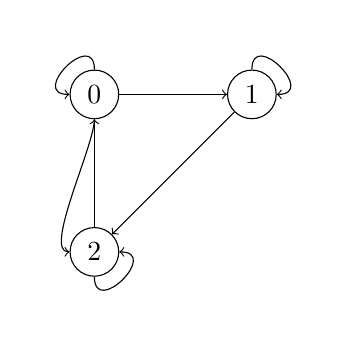
\begin{tikzpicture}[main/.style={draw,circle},node distance={2cm}]
                \node[main](0){$0$};
                \node[main](1)[right of=0]{$1$};
                \node[main](2)[below of=0]{$2$};
                \draw[->](0) to [out=90,in=180,looseness=3] (0);
                \draw[->](0) -- (1);
                \draw[->](0) to [out=270,in=180,looseness=0.5] (2);
                \draw[->](1) to [out=90,in=0,looseness=3] (1);
                \draw[->](1) -- (2);
                \draw[->](2) to [out=270,in=0,looseness=3] (2);
                \draw[->](2) -- (0);
            \end{tikzpicture}
        \end{center}
        Thus $\left\lbrace 0,1,2 \right\rbrace$ is the only communication class of the DTMC; in other words, the DTMC is irreducible.
    \end{subproof}

    \ex Consider a DTMC with TPM
    \begin{equation*}
        P =
        \begin{bmatrix}
        	0 & 1 & 0 & 0 \\
        	0 & 0 & 1 & 0 \\
        	0 & 0 & 0 & 1 \\
        	\frac{1}{2} & 0 & \frac{1}{2} & 0 \\
        \end{bmatrix}.
    \end{equation*}
    Find the communication classes of this DTMC.

    \begin{subproof}[Answer]
        By drawing a state transition diagram, it is clear that the DTMC is irreducible.
    \end{subproof}

    \ex Consider a DTMC with TPM
    \begin{equation*}
        P =
        \begin{bmatrix}
        	\frac{1}{3} & \frac{2}{3} & 0 & 0 \\
        	\frac{1}{2} & \frac{1}{4} & \frac{1}{8} & \frac{1}{8} \\
        	0 & 0 & 1 & 0 \\
        	\frac{3}{4} & \frac{1}{4} & 0 & 0 \\
        \end{bmatrix}.
    \end{equation*}
    Find the communication classes of this DTMC.

    \begin{subproof}[Answer]
        Observe that the state transition diagram is
        \begin{center}
            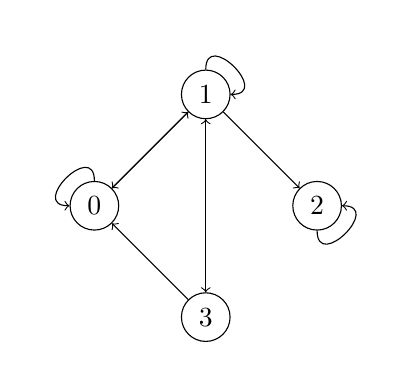
\begin{tikzpicture}[main/.style={draw,circle},node distance={2cm}]
                \node[main](0){$0$};
                \node[main](1)[above right of=0]{$1$};
                \node[main](2)[below right of=1]{$2$};
                \node[main](3)[below right of=0]{$3$};
                \draw[->](0) to [out=90,in=180,looseness=3] (0);
                \draw[->](0) -- (1);
                \draw[->](1) to [out=90,in=0,looseness=3] (1);
                \draw[->](1) -- (0);
                \draw[->](1) -- (2);
                \draw[->](1) -- (3);
                \draw[->](2) to [out=270,in=0,looseness=3] (2);
                \draw[->](3) -- (0);
                \draw[->](3) -- (1);
            \end{tikzpicture}
        \end{center}
        Thus $\left\lbrace 0,1,3 \right\rbrace, \left\lbrace 2 \right\rbrace$ are the communication classes of the DTMC.
    \end{subproof}







































    

\end{document}
